\documentclass[12pt]{report}
\usepackage[margin=2.5cm]{geometry}
\usepackage[utf8]{vietnam}
\usepackage{pdfpages}
\usepackage{fancyhdr}
\usepackage{graphicx}
\usepackage{hyperref}
\usepackage{float}

% Change format of page
\pagestyle{fancy}
\fancyhf{}
\fancyhead{}
\fancyfoot{}
\fancyhead[L]{Big Data}
\fancyfoot[L]{Nhóm 6 - KSTN-CNTT-K60}
\fancyfoot[R]{\thepage}
\renewcommand{\headrulewidth}{1pt}
\renewcommand{\footrulewidth}{1pt}
\usepackage{etoolbox}
\patchcmd{\chapter}{\thispagestyle{plain}}{\thispagestyle{fancy}}{}{}

% Link color setup
\hypersetup{
	colorlinks = true,
	linkcolor = black,
	citecolor = blue
}

\usepackage{caption}
\captionsetup[figure]{labelfont={it}}

\renewcommand\thesection{\arabic{section}}

\begin{document}
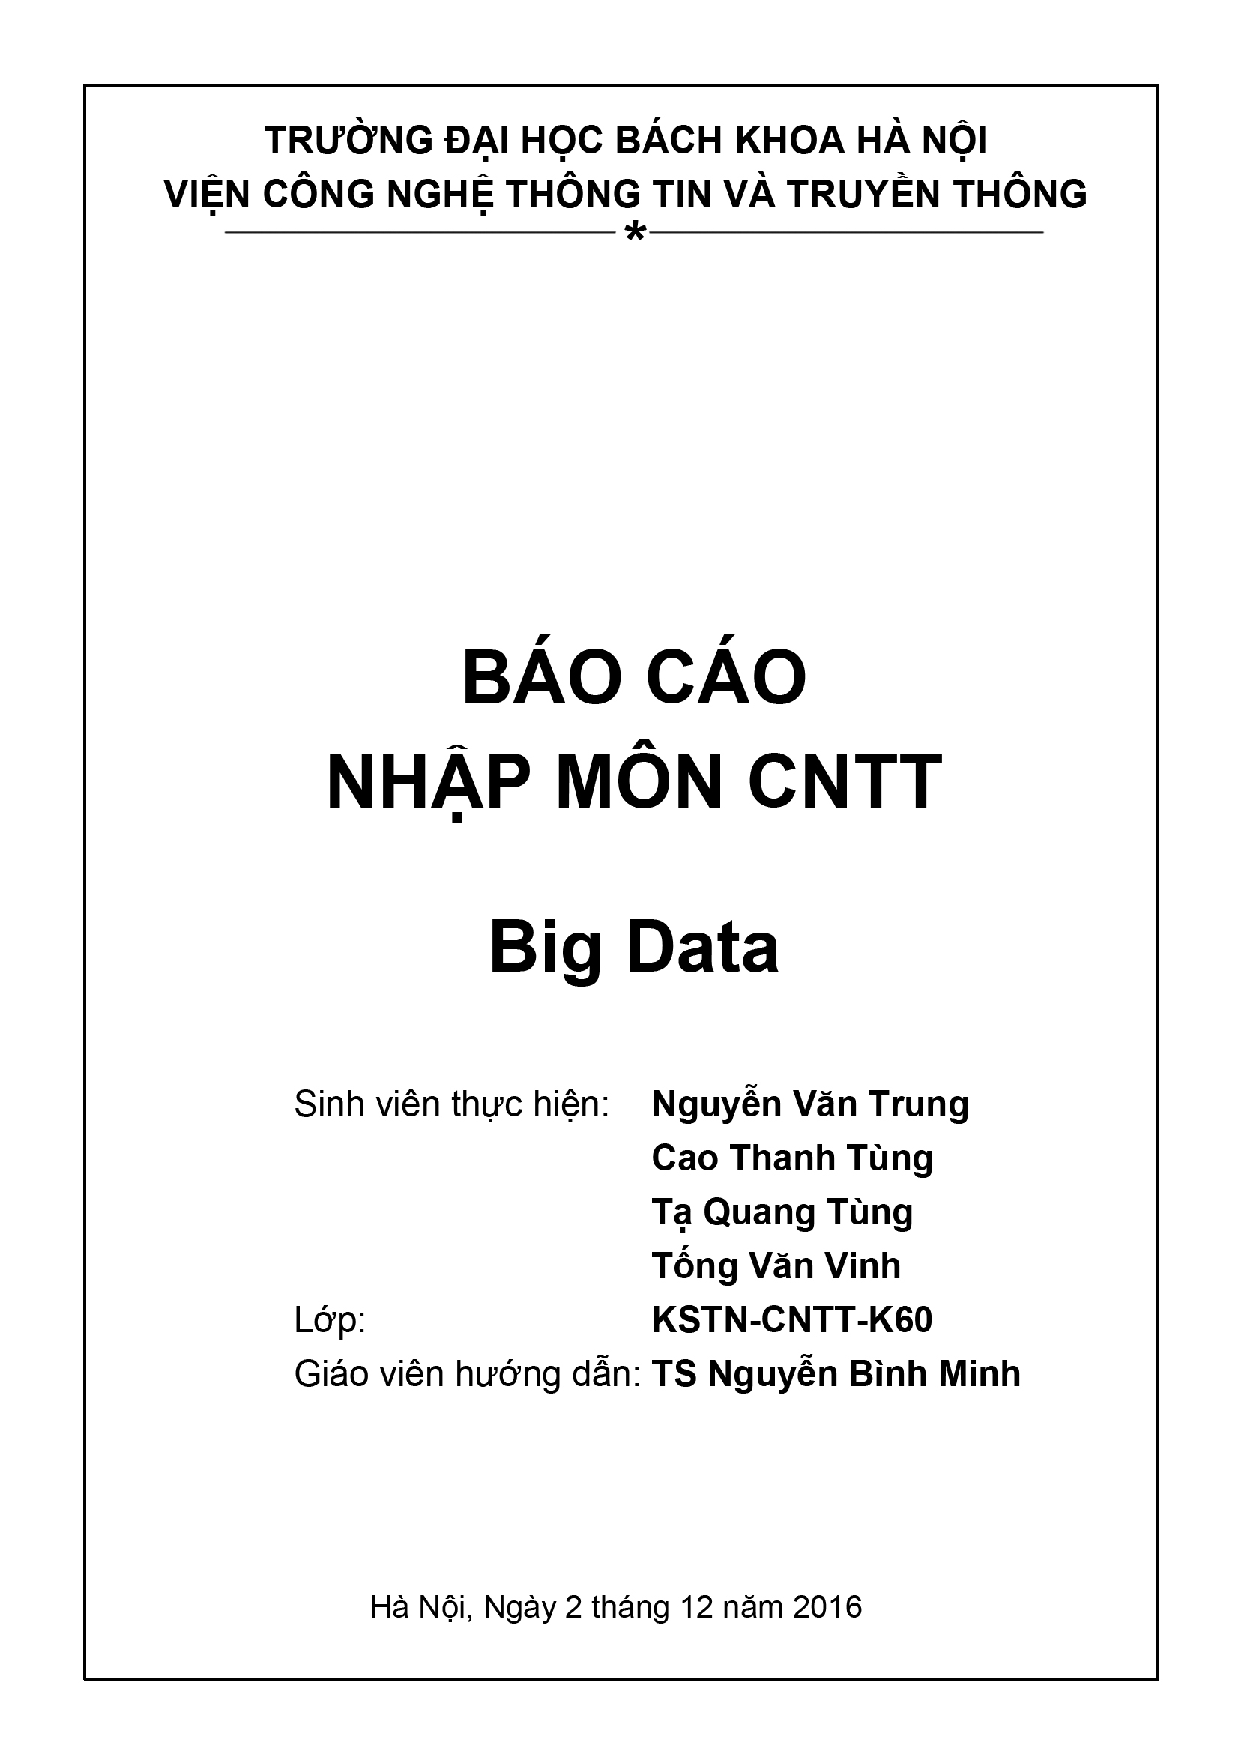
\includepdf{report.pdf}
\newpage
\setcounter{page}{1}
\tableofcontents
\newpage
\chapter*{Lời nói đầu}
\addcontentsline{toc}{chapter}{Lời nói đầu}
Con người từ thủa sơ khai đã luôn ao ước có thể nghiên cứu và học hỏi nhiều hơn để bằng cách nào đó có thể dự đoán chính xác (hoặc gần đúng) những điều sẽ xảy đến trong tương lai. Và cho đến tận bây giờ ao ước đó vẫn còn rất cháy bỏng. Nhưng điều kiện kiên quyết để có thể dự đoán chính xác tương lai là nắm rõ mọi chi tiết của thực tại. Và ai cũng biết rằng, điều đó, với những vấn đề trong cuộc sống, rõ ràng là không thể. Nhưng thay vì chúng ta biết tất cả về thực tại, chúng ta có thể hài lòng hơn khi biết và hiểu nhiều hơn về thực tại. Không cần tất cả, chỉ cần đủ nhiều tri thức, xác suất để giải quyết tốt những bài toán thực tế cũng như dự đoán trước tương lai có thể đủ lớn để chúng ta chấp nhận được. Và để có nhiều tri thức hơn, ta phải có nhiều dữ liệu hơn, việc thu thập và xử lý một lượng lớn dữ liệu đang trở thành một vấn đề, thậm trí là một trào lưu mà cả thế giới đang chú ý đến, đó chính là bigdata. 

Nhiều dữ liệu hơn không những giúp ta thấy nhiều hơn, nhiều dữ liệu hơn còn giúp ta thấy được những điều mới, mang đến một góc nhìn tốt hơn, cho phép ta thấy khác đi. Chúng ta chắc hẳn đã từng nghe về khái niệm Big Data. Không thể phủ nhận rằng có nhiều sự thổi phồng xung quanh khái niệm trên, và điều đó thật đáng tiếc, vì Bigdata là một công cụ cực kì quan trọng mà nhờ đó, xã hội sẽ trở nên tiến bộ hơn. Trong quá khứ, chúng ta thường nhìn vào những dữ liệu nhỏ, tìm hiểu ý nghĩa của chúng, để cố gắng hiểu về thế giới, và giờ, ta có nhiều dữ liệu hơn, nhiều hơn bao giờ hết. Những gì ta biết là khi có một lượng lớn dữ liệu, ta có thể làm những điều mà trước kia không thể. 

Dữ liệu lớn rất quan trọng và mới mẻ, và đó có thể là cách duy nhất mà hành tinh này sẽ đối phó với những thử thách toàn cầu: Đảm bảo thức ăn cho mọi người, cung cấp dịch vụ y tế, cung cấp năng lượng, điện, và đảm bảo người dân không bị thiêu rụi bởi sự nóng lên toàn cầu. Tất cả nhờ vào việc sử dụng dữ liệu hiệu quả. Xuất phát từ những lợi ích lớn lao đó, nhóm chúng em chọn đề tài tìm hiểu về Bigdata.
Bài báo cáo sẽ đề cập đến khái niệm về Bigdata cũng như những lợi ích mà nó đem lại. Ngoài ra, còn đi vào tìm hiểu cơ sở khoa học, những khó khăn và đặc thù trong việc xử lý dữ liệu lớn mà phải thực hiện khác so với những công việc chúng ta thường làm với dữ liệu nhỏ.

Để hoàn thành được bài tập lớn này, nhóm chúng em đã tích cực tìm hiểu thông tin sách báo cũng như  từ các nguồn đáng tin cậy trên internet. Đồng thời cùng với sự kết hợp ăn ý và phân chia công việc hợp lý, cả nhóm đã cùng nhau hoàn thành bài tập lớn với tất cả tâm huyết và đam mê nghiên cứu. Xin được gửi lời cảm ơn chân thành đến Thầy Nguyễn Bình Minh , Giảng viên Khoa Hệ thống thông tin Trường Đại học Bách Khoa Hà Nội - đã hết lòng giúp đỡ, hướng dẫn, chỉ dạy tận tình để nhóm em hoàn thành được đề tài này.
\newpage
\begin{flushright}
\bfseries
Hà Nội, Ngày 2 tháng 12 năm 2016 \\
\vspace{0.5cm}
Nhóm 6, Lớp KSTN-CNTT-K60 \\
(Danh sách thành viên ký tên) \\
\vspace{4mm}
NGUYỄN VĂN TRUNG \\
\vspace{13mm}
CAO THANH TÙNG \\
\vspace{13mm}
TẠ QUANG TÙNG \\
\vspace{13mm}
TỐNG VĂN VINH
\newpage

\end{flushright}

\chapter*{Nội dung}
\addcontentsline{toc}{chapter}{Nội dung}
\section{Khái quát về Big Data}
\subsection{Big Data là gì?}

Big Data là thuật ngữ dùng để chỉ một tập hợp dữ liệu rất lớn và rất phức tạp đến nỗi những công cụ, ứng dụng xử lí dữ liệu truyền thống không thể nào đảm đương được. \cite{definition}

\begin{figure}[H]
\centering
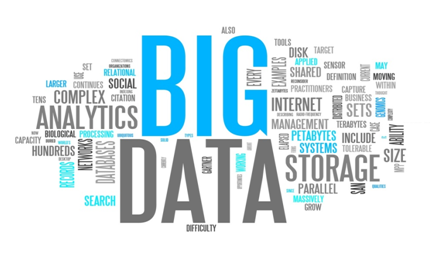
\includegraphics[scale=1]{big_data.png}
\caption{ }
\end{figure}

Kích cỡ của Big Data đang từng ngày tăng lên, và tính đến năm 2012 thì nó có thể nằm trong khoảng vài chục terabyte cho đến nhiều petabyte (1 petabyte = 1024 terabyte) chỉ cho một tập hợp dữ liệu mà thôi.

\subsection{Đặc điểm nổi trội của Big Data}
\begin{itemize}
\item \textbf{Dung lượng (Volume)}: Dung lượng của Big Data đang tăng lên mạnh mẽ từng ngày. Theo tài liệu của Intel vào tháng 9/2013, cứ mỗi 11 giây, 1 petabyte dữ liệu được tạo ra trên toàn thế giới, tương đương với một đoạn video HD dài 13 năm. 
\item \textbf{Tốc độ (Velocity)}: là tốc độ mà tại đó dữ liệu được phân tích bởi các công ty để cung cấp một trải nghiệm người dùng tốt hơn. Với sự ra đời của các kỹ thuật, công cụ, ứng dụng lưu trữ, nguồn dữ liệu liên tục được bổ sung với tốc độ nhanh chóng. Tổ chức McKinsey Global ước tính lượng dữ liệu đang tăng trưởng với tốc độ 40%/năm, và sẽ tăng 44 lần từ năm 2009 đến 2020.
\item \textbf{Tính đa dạng (Variety)}: Dữ liệu được thu thập từ nhiều nguồn khác nhau, từ các thiết bị cảm biến, thiết bị di động, qua mạng xã hội .v.v…
\item \textbf{Giá trị (Value)}: là quá trình trích xuất các giá trị to lớn đang tiềm ẩn trong các bộ dữ liệu khổng lồ. Đây là đặc trưng quan trọng nhất bởi các thông tin trích xuất được từ việc phân tích Dữ liệu lớn có thể được sử dụng trong rất nhiều lĩnh vực như kinh doanh, nghiên cứu khoa học, y học, vật lý…
\end{itemize}

\subsection{Big Data có vai trò lợi ích gì?}
Big Data chứa trong nó rất nhiều thông tin quý giá mà nếu trích xuất thành công, nó sẽ giúp rất nhiều cho việc:
\begin{itemize}
	\item[+] Kinh doanh.
	\item[+] Nghiên cứu khoa học.
	\item[+] Dự đoán các dịch bệnh sắp phát sinh.
	\item[+] Dự đoán tỉ lệ thất nghiệp, xu hướng nghề nghiệp.
	\item[+] Xác định điều kiện giao thông theo thời gian thực.
	\item[+] …
\end{itemize}

\begin{figure}[H]
\centering
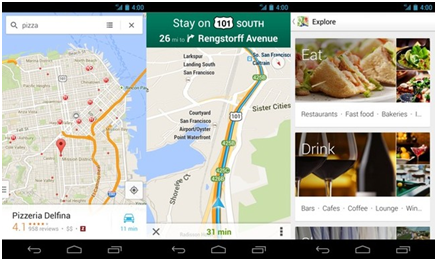
\includegraphics[scale=1]{util.png}
\caption{\it Giao thông thời gian thực}
\end{figure}
Nhìn chung, có bốn lợi ích mà Big Data có thể mang lại: 
\begin{itemize}
	\item[+] Cắt giảm chi phí.
	\item[+] Giảm thời gian.
	\item[+] Tăng thời gian phát triển và tối ưu hóa sản phẩm.
	\item[+] Hỗ trợ con người đưa ra những quyết định đúng và hợp lý hơn. (những điều này thể hiện như thế nào, thì ở những ví dụ sẽ được làm rõ)
\end{itemize}

\subsection{Tại sao Big Data đang trở thành một xu thế?}
Theo các nhà phân tích, ngành công nghiệp phần mềm đã giúp hàng nghìn người trở thành triệu phú, tỷ phú và vòng xoay này đang lặp lại với Big Data. Ngược dòng lịch sử, trước khi phát minh ra máy tính cá nhân (PC), các công ty phải chi hàng triệu USD cho các máy tính cồng kềnh để xử lý dữ liệu. Apple và Microsoft đã thay đổi điều đó bằng việc đưa máy tính vào mọi nhà. Với Big Data cũng vậy, khi giá của những bộ nhớ lớn, xử lý tốc độ cao giảm xuống, các công ty có thể truy cập khối lượng dữ liệu lớn cả bên trong và bên ngoài công ty, từ đó đưa ra đánh giá chính xác về thị trường, nắm bắt cơ hội và thu lợi nhuận.  Vì vậy, Big Data là câu chuyện thời thượng, thu hút sự quan tâm đặc biệt của giới kinh doanh công nghệ toàn thế giới.

\section{Những ví dụ về Big Data}
Có rất nhiều ví dụ về Big Data, tuy nhiên chúng tôi sẽ chọn những ví dụ cho mọi người dễ hình dung nhất về vấn đề này.

\subsection{Thí nghiệm về máy gia tốc hạt lớn (LHC) ở Châu Âu}
Khi các thí nghiệm trên máy được tiến hành, kết quả sẽ được ghi nhận bởi 150 triệu cảm biến với nhiệm vụ truyền tải dữ liệu khoảng 40 triệu lần mỗi giây. Kết quả là nếu như LHC ghi nhận hết kết quả từ mọi cảm biến thì luồng dữ liệu sẽ trở nên vô cùng lớn, có thể đạt đến 150 triệu petabyte mỗi năm, hoặc 500 exabyte mỗi ngày, cao hơn 200 lần so với tất cả các nguồn dữ liệu khác trên thế giới gộp lại.

\begin{figure}[H]
\centering
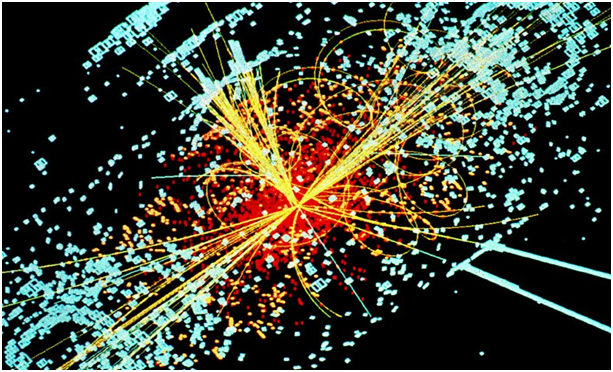
\includegraphics[scale=1]{lhc.png}
\caption{\it Đây là kết quả mô phỏng của một vụ va chạm giữa các hạt sơ cấp trong máy gia tốc LHC, có rất rất nhiều thông tin cần phải ghi nhận trong mỗi vụ chạm như thế này}
\end{figure}

Trong mỗi giây như thế lại có đến khoảng 600 triệu vụ va chạm giữa các hạt vật chất diễn ra, nhưng sau khi chọn lọc lại từ khoảng 99,999\% các luồng dữ liệu đó, chỉ có tầm 100 vụ va chạm là được các nhà khoa học quan tâm. Điều này có nghĩa là cơ quan chủ quản LHC phải tìm những biện pháp mới để quản lý và xử lí hết mớ dữ liệu khổng lồ này.

\subsection{Mối quan hệ giữa bigdata và Trí tuệ nhân tạo}
Một trong những lĩnh vực ấn tượng nhất mà khái niệm này đang diễn ra là trong lĩnh vực học máy. Máy học là một nhánh của trí tuệ nhân tạo mà bản thân nó lại là một nhánh của khoa học máy tính. Ý tưởng chung là thay vì phải hướng dẫn máy tính những gì phải làm, chúng ta sẽ chỉ ném dữ liệu liên quan đến vấn đề và bảo máy tính tự tính toán. Và để bạn hiểu được vấn đề này, hãy cùng nhìn lại nguồn gốc của nó. Vào những năm 1950, một nhà khoa học máy tính của IBM tên Arthur Samuel đã viết một chương trình máy tính để ông ấy có thể chơi cờ với máy nó. Ông ấy chơi và liên tục thắng. Bởi vì máy tính chỉ đơn giản biết một nước đi thế nào là đúng luật. Còn Arthur Samuel không chỉ hiểu luật chơi mà còn biết chiến thuật và mưu mẹo nữa. Arthur Samuel tiếp tục nâng cấp cho phần mềm đánh cờ bằng cách cài đặt thêm một chương trình con ghi lại xác suất những nước đi quen thuộc thường dẫn đến chiến thắng. Tuy nhiên, ông vẫn luôn thắng mỗi khi đánh cờ với chiếc máy tính của mình. Cuối cùng ông ta để máy tính tự chơi cờ với chính nó. Nó tự chơi cờ, nó thu thập nhiều dữ liệu hơn. Nó thu thập nhiều dữ liệu hơn, nó tăng độ chính xác về khả năng dự đoán. Và khi Arthur Samuel quay lại và đánh cờ với máy, ông ấy không thể thắng được chiếc máy tính của mình nữa. Vậy là Arthur Samuel đã tạo ra một chương trình vượt qua khả năng của ông ấy trong một việc mà ông ấy dạy nó. Và ý tưởng này về học máy đang được ứng dụng ở mọi nơi. 

Máy học là nền tảng cơ bản của rất nhiều thứ chúng ta làm trên mạng: Các công cụ tìm kiếm, thuật toán cá nhân hóa của amazon, máy tính dịch thuật, hệ thống xác nhận giọng nói. Gần đây các nhà nghiên cứu đã tìm hiểu về các vấn đề sinh thiết. Sinh thiết ung thư, và họ đã nhờ máy tính xác định, bằng cách nhìn vào dữ liệu và chỉ số sống sót để xác nhận rằng những tế bào này có thật sự bị ung thư hay không. Và thật ngạc nhiên là máy tính có thể chẩn đoán chính xác đến bất ngờ, thậm chí có thể đưa ra lộ trình chữa trị hiệu quả hơn của các bác sĩ!

\subsection{Các ví dụ khác}
Khi Sloan Digital Sky Sruver, một trạm quan sát vũ trụ đặt tại New Mexico, bắt đầu đi vào hoạt động hồi năm 2000, sau một vài tuần nó đã thu thập dữ liệu lớn hơn tổng lượng dữ liệu mà ngành thiên văn học đã từng thu thập trong quá khứ, khoảng 200GB mỗi đêm và hiện tổng dung lượng đã đạt đến hơn 140 terabyte. Đài quan sát LSST để thay thế cho SDSS dự kiến khánh thành trong năm 2016 thì sẽ thu thập lượng dữ liệu tương đương như trên nhưng chỉ trong vòng 5 ngày.

Hoặc như công tác giải mã di truyền của con người. Trước đây công việc này mất đến 10 năm để xử lí, còn bây giờ người ta chỉ cần một tuần là đã hoàn thành. 

Còn Trung tâm giả lập khí hậu của NASA thì đang chứa 32 petabyte dữ liệu về quan trắc thời tiết và giả lập trong siêu máy tính của họ.

Việc lưu trữ hình ảnh, văn bản và các nội dung đa phương tiện khác trên Wikipedia cũng như ghi nhận hành vi chỉnh sửa của người dùng cũng cấu thành một tập hợp Big Data.

\begin{figure}[H]
\centering
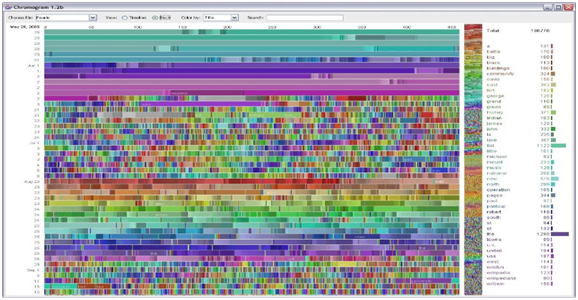
\includegraphics[scale=1]{wiki.png}
\caption{\it Hoạt động của người dùng Wikipedia được mô hình hóa và với kích thước hàng terabyte, đây cũng có thể được xem là một dạng Big Data}
\end{figure}

\subsection{Thêm một vài thông tin cập nhật}
Theo tài liệu của Intel vào tháng 9/2013, hiện nay thế giới đang tạo ra 1 petabyte dữ liệu trong mỗi 11 giây và nó tương đương với một đoạn video HD dài 13 năm. Bản thân các công ty, doanh nghiệp cũng đang sở hữu Big Data của riêng mình, chẳng hạn như trang bán hàng trực tuyến eBay thì sử dụng hai trung tâm dữ liệu với dung lượng lên đến 40 petabyte để chứa những truy vấn, tìm kiếm, đề xuất cho khách hàng cũng như thông tin về hàng hóa của mình.

Nhà bán lẻ online Amazon.com thì phải xử lí hàng triệu hoạt động mỗi ngày cũng như những yêu cầu từ khoảng nửa triệu đối tác bán hàng. Amazon sử dụng một hệ thống Linux và hồi năm 2005, họ từng sở hữu ba cơ sở dữ liệu Linux lớn nhất thế giới với dung lượng là 7,8TB, 18,5TB và 24,7TB. 

Tương tự, Facebook cũng phải quản lí 50 tỉ bức ảnh từ người dùng tải lên, YouTube hay Google thì phải lưu lại hết các lượt truy vấn và video của người dùng cùng nhiều loại thông tin khác có liên quan.

\subsection{Tiện ích với Big Data}
Nếu để ý một chút, bạn sẽ thấy khi mua sắm online trên eBay, Amazon, Tiki, Lazada hoặc những trang tương tự, trang này cũng sẽ đưa ra những sản phẩm gợi ý tiếp theo cho bạn, ví dụ khi xem điện thoại, nó sẽ gợi ý cho bạn mua thêm ốp lưng, pin dự phòng; hoặc khi mua áo thun thì sẽ có thêm gợi ý quần jean, dây nịt... Do đó, nghiên cứu được sở thích, thói quen của khách hàng cũng gián tiếp giúp doanh nghiệp bán được nhiều hàng hóa hơn.

\begin{figure}[H]
\centering
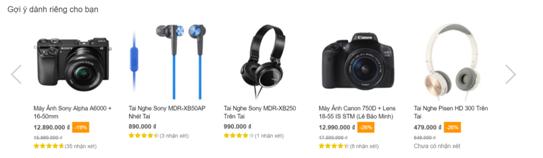
\includegraphics[scale=1]{ebay.png}
\caption{\it Tiện ích của Big Data}
\end{figure}

Vậy những thông tin về thói quen, sở thích này có được từ đâu? Chính là từ lượng dữ liệu khổng lồ mà các doanh nghiệp thu thập trong lúc khách hàng ghé thăm và tương tác với trang web của mình. Chỉ cần doanh nghiệp biết khai thác một cách có hiệu quả Big Data thì nó không chỉ giúp tăng lợi nhuận cho chính họ mà còn tăng trải nghiệm mua sắm của người dùng, chúng ta có thể tiết kiệm thời gian hơn nhờ những lời gợi ý so với việc phải tự mình tìm kiếm.

Người dùng cuối chúng ta sẽ được hưởng lợi cũng từ việc tối ưu hóa như thế, chứ bản thân chúng ta thì khó mà tự mình phát triển hay mua các giải pháp để khai thác Big Data bởi giá thành của chúng quá đắt, có thể đến cả trăm nghìn đô. Ngoài ra, lượng dữ liệu mà chúng ta có được cũng khó có thể xem là “Big” nếu chỉ có vài Terabyte sinh ra trong một thời gian dài.

Xa hơi một chút, ứng dụng được Big Data có thể giúp các tổ chức, chính phủ dự đoán được tỉ lệ thất nghiệp, xu hướng nghề nghiệp của tương lai để đầu tư cho những hạng mục đó, hoặc cắt giảm chi tiêu, kích thích tăng trưởng kinh tế, v.v... thậm chí là ra phương án phòng ngừa trước một dịch bệnh nào đó, giống như trong phim World War Z, nước Israel đã biết trước có dịch zombie nên đã nhanh chóng xây tường thành ngăn cách với thế giới bên ngoài.

Mà cũng không cần nói đến tương lai phim ảnh gì cả, vào năm 2009, Google đã sử dụng dữ liệu Big Data của mình để phân tích và dự đoán xu hướng ảnh hưởng, lan truyền của dịch cúm H1N1 đấy thôi. Dịch vụ này có tên là Google Flu Trends. Xu hướng mà Google rút ra từ những từ khóa tìm kiếm liên quan đến dịch H1N1 đã được chứng minh là rất sát với kết quả do hai hệ thống cảnh báo cúm độc lập Sentinel GP và HealthStat đưa ra. Dữ liệu của Flu Trends được cập nhật gần như theo thời gian thực và sau đó sẽ được đối chiếu với số liệu từ những trung tâm dịch bệnh ở nhiều nơi trên thế giới.

\begin{figure}[H]
\centering
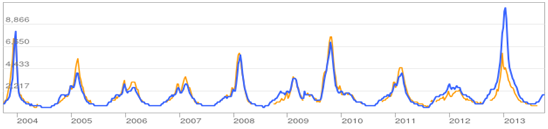
\includegraphics[scale=1]{graph.png}
\caption{\it Đường màu xanh là dự đoán của Google Flu Trends dựa trên số từ khóa tìm kiếm liên quan đến các dịch cúm, màu vàng là dữ liệu do cơ quan phòng chống dịch của Mỹ đưa ra.}
\end{figure}

\section{Các công cụ khai thác Big Data}
\subsection{Cụm máy tính (Computer Cluster)}
Với một lượng dữ liệu lớn như vậy thì ta cần sử dụng những máy tính có sức mạnh lớn để xử lý nó. Một trong những kiến trúc phổ biến nhất đối với một siêu máy tính (chiếm tới 80\% thị phần siêu máy tính, theo TOP500 \cite{top500}) hay một trung tâm dữ liệu đó là kiến trúc cluster.
\begin{figure}[H]
\centering
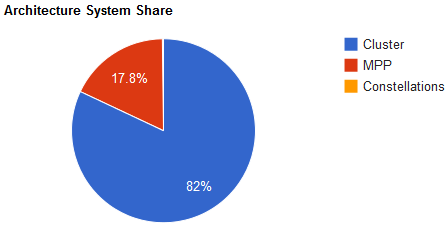
\includegraphics[scale=1]{top500.png}
\caption{\it Thị phần kiến trúc siêu máy tính}
\end{figure}

Một cụm máy tính (computer cluster) là một tập hợp những máy tính hoạt động cùng nhau, thường được kết nối với nhau thông qua một mạng LAN tốc độ rất cao, thường được đặt gần nhau trong cùng một trung tâm dữ liệu. Mỗi node trong cluster là một máy tính chạy một hệ điều hành, trên một phần cứng riêng biệt. Ở nhiều khía cạnh, có thể coi một cụm máy tính là một hệ thống đơn nhất. 

\begin{figure}[H]
\centering
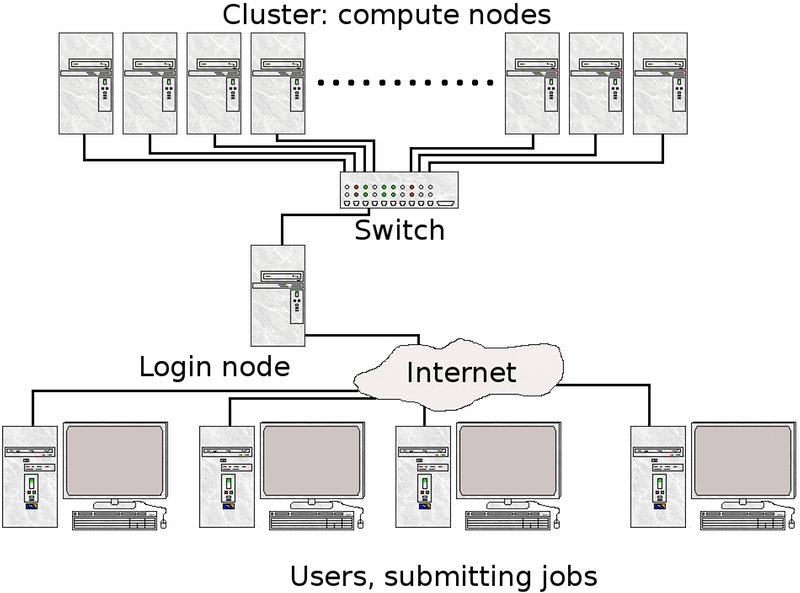
\includegraphics[width=9cm]{cluster.png}
\caption{\it Ví dụ về kiến trúc cluster}
\end{figure}

\begin{figure}[H]
\centering
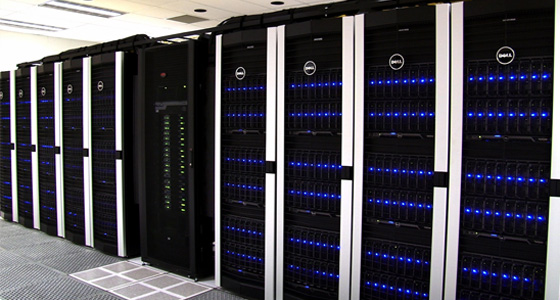
\includegraphics[width=\textwidth]{cluster.jpg}
\caption{\it Trung tâm dữ liệu dưới dạng cluster}
\end{figure}

Kiến trúc cluster là một trong những kiến trúc mạnh mẽ với chi phí xây dựng hiệu quả hơn nhiều kiến trúc khác. Cụm máy tính cung cấp sức mạnh tính toán nhờ sử dụng tính toán song song, đồng thời có khả năng chịu lỗi cao – cluster vẫn có thể hoạt động khi một trong các node bị hỏng, nhờ đó đem lại tính luôn sẵn sàng cho hệ thống. Đồng thời đây là một kiến trúc phổ biến dành cho việc giải quyết các vấn đề trong Big Data.

\subsection{Công nghệ Hadoop}
\subsubsection{Tổng quan về Hadoop}

Nhắc tới Big Data ta không thể không nhắc tới Hadoop, nó phổ biến đến mức nhiều khi Hadoop còn được dùng đồng nghĩa với Big Data. Hadoop được tạo bởi Doug Cutting, nhà sáng lập của Apache Lucene.

Hadoop, xuất bản đầu tiên vào 10/12/2011\cite{hadoop}, là một framework mã nguồn mở phát triển bởi Apache Software Foundation được sử dụng cho lưu trữ và xử lý phân tán trên một lượng lớn dữ liệu. Hadoop được viết bằng ngôn ngữ Java và hoạt động trên một cụm máy tính,  được phát triển nhờ ý tưởng từ hai bài báo nổi tiếng của Google về Google File System (GFS) và MapReduce. 

\subsubsection{Hệ thống file phân tán Hadoop (Hadoop Distributed File System – HDFS)}

Làm việc một lượng dữ liệu lớn như vậy thì vấn đề đầu tiên đặt ra là phải lưu trữ nó như thế nào? Việc lưu trữ bằng cách thông thường với Big Data không thể đáp ứng được. Một máy tính không thể lưu trữ lượng thông tin lớn đến cả trăm Terabyte như vậy. Đồng thời nếu sử dụng cluster với cách lưu trữ thông thường (Không có cơ chế bảo vệ dữ liệu) thì khi một node bị hỏng, dữ liệu bị mất là điều khó tránh khỏi.

Để đáp ứng được nhu cầu lưu trữ như vậy, Hadoop đi cùng với hệ thống file phân tán gọi là HDFS. Các ứng dụng trên Hadoop sử dụng HDFS. HDFS được thiết kế để lưu trữ các tệp dữ liệu rất lớn, chạy trên các cluster, với các đặc tính:

\begin{itemize}
\item \textit{Sử dụng với những file rất lớn}: “Rất lớn” ở đây nghĩa rằng file có kích thước tính bằng MB, GB hoặc TB. Có những cụm máy tính chạy Hadoop ngày nay có lượng dữ liệu lưu trữ lên đến hàng Petabyte (1024 Terabyte).

\item \textit{Truy cập dưới dạng stream}: HDFS được xây dựng dựa trên ý tưởng rằng cách hiệu quả nhất để xử lý dữ liệu là “ghi một lần – đọc nhiều lần”, hay là tối ưu hóa việc đọc dữ liệu. Một bộ dữ liệu thường được sản sinh hay sao chép từ một nguồn nào đó, và rất nhiều những phép toán phân tích được thực hiện trên nó theo thời gian. Mỗi phép toán phân tích sẽ yêu cầu một phần, nếu không phải toàn bộ dữ liệu đã thu thập. Vì vậy việc đọc toàn bộ dữ liệu xảy ra thường xuyên hơn nhiều việc ghi.

\item \textit{Sử dụng Commodity Hardware}: Hadoop không yêu cầu những phần cứng đắt tiền, có tính tin cậy cao. Nó được thiết kế để chạy trên một cluster của các Commodity Hardware (Những phần cứng phổ biến mà có thể đến từ nhiều nhà sản xuất khác nhau, không phải những phần cứng được thiết kế chuyên biệt như các kiến trúc khác). Những phần cứng này có tỉ lệ hỏng hóc cao nếu so với một cluster lớn. HDFS được thiết kế để làm việc với những hỏng hóc như vậy mà không làm ngắt quãng việc xử lý đối với người sử dụng (client). 
\end{itemize}

Những khái niệm trong HDFS:
\begin{itemize}
\item[+] \textbf{Block}: Ổ cứng có những block, là kích thước nhỏ nhất mà có thể đọc được mỗi lần, thông thường là 512 byte. HDFS cũng vậy, nhưng block trong HDFS có kích thước lớn hơn rất nhiều – mặc định là 128 MB. Tuy nhiên có sự khác biệt là một file có kích thước nhỏ hơn một block trong HDFS thì không chiếm giữ toàn bộ nó. Mục đích của việc block trong HDFS rất lớn là để giảm việc dịch chuyển giữa các vùng trong ổ cứng – khi kết hợp với phương pháp lưu trữ tạm thời trong RAM. Block cung cấp một lớp trìu tượng đối với dữ liệu trong ổ cứng. Đồng thời nó là trung tâm của việc sao chép dữ liệu: Hadoop duy trì một số lượng cố định những bản sao chép của một block và phân bố nó trải rộng trên các node của cluster. 

\item[+] \textbf{Namenode và Datanode}: Một node trong cluster chạy HDFS sẽ chiếm một trong hai vai trò, một là master (namenode) – node trung tâm, có ảnh hưởng lớn đến các node khác, và slave (datanode) – node hoạt động dưới sự quản lý của master. Namenode quản lý toàn bộ không gian tên của HDFS. Nó quản lý toàn bộ cây thư mục, những metadata cho tất cả các file trong HDFS. Những thông tin này được namenode được lưu trữ lâu dài trong ổ cứng của nó. Metadata của từng file lưu trữ thông tin của file đó như tên file, vị trí của các datanode, vị trí của block chứa file.

Datanode là những node mà dữ liệu (block) thực sự được lưu trữ. Chúng lưu trữ và lấy block trong ổ cứng khi được yêu cầu, báo cáo định kì về cho namenode danh sách những block cua mình. Nếu không có namenode, toàn bộ hệ thống file không thể được sử dụng. Vì vậy, namenode thường là nơi chứa máy tính có độ tin cậy và sức mạnh cao nhất trong cluster. Và để  chống lại những sự cố xảy ra ở namenode, HDFS có thể back up những dữ liệu của namenode một cách định kì, hoặc sử dụng một namenode thứ hai để tránh hỏng hóc xảy ra ở namenode chính. 

\begin{figure}[H]
\centering
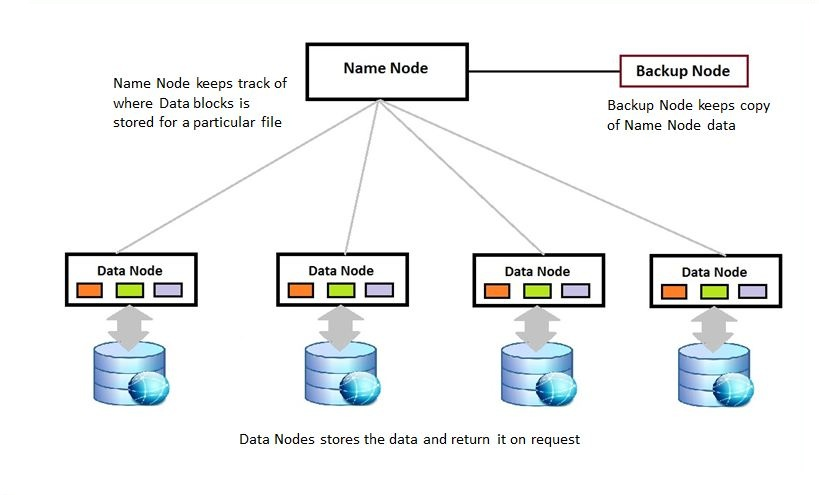
\includegraphics[width=\textwidth]{namenode.jpg}
\caption{\it Namenode và Datanode}
\end{figure}
\end{itemize}

\textbf{Hoạt động của HDFS}
\begin{itemize}
\item \textbf{Đọc file}: Việc đọc file bắt đầu khi client gọi hàm open, qua nó, client gửi yêu cầu dữ liệu cho namenode. Namenode sau đó trả về địa chỉ của các datanode mà lưu trữ block của file cần truy cập. Client lựa chọn node gần nhất trong các datanode để đọc dữ liệu. Nếu bản thân client là datanode đó, client sẽ đọc dữ liệu từ chính ổ cứng của mình. Trong trường hợp datanode được yêu cầu dữ liệu không đáp lại, client sẽ báo ngược trở lại namenode rằng datanode đó đã có sự cố, đồng thời cố gắng truy cập những datanode còn lại. Việc đọc dữ liệu sau đó sẽ thông qua đường truyền dữ liệu mạng như thông thường giữa client và datanode. Tất cả những thao tác đó được gói gọn trong API cung cấp bởi Hadoop, với giao diện giống như chuẩn POSIX thông thường.

\begin{figure}[H]
\centering
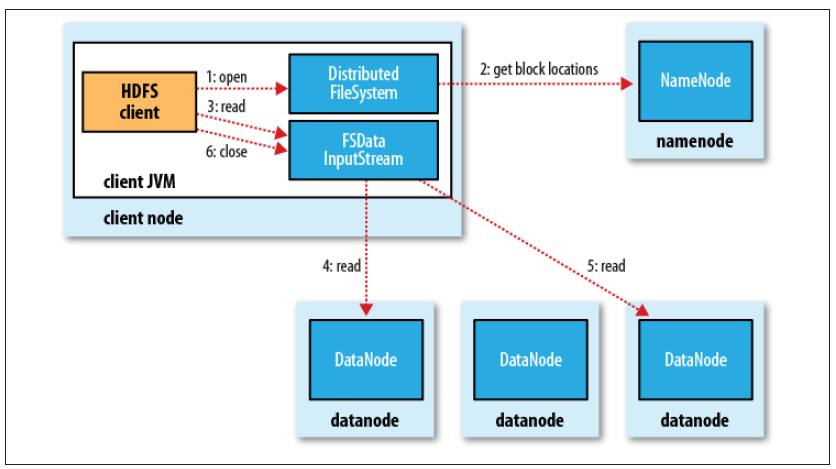
\includegraphics[width=\textwidth]{read.png}
\caption{\it Đọc dữ liệu trên HDFS \cite{read}}
\end{figure}

\item \textbf{Ghi file}: Việc ghi dữ liệu bắt đầu khi client gọi hàm create, yêu cầu cho namenode tạo một file mới trong cây thư mục của nó. Namenode sau đó tạo  một bản ghi của file vừa mới tạo. Client yêu cầu namenode cấp phát một danh sách các datanode để lưu trữ file. Client sẽ ghi dữ liệu vào datanode thứ nhất, đồng thời datanode thứ nhất chuyển tiếp dữ liệu cho datanode thứ hai trong danh sách, tạo nên một cơ chế đường ống, cứ như vậy cho đến datanode cuối cùng – số lượng datanode tương ứng với số lượng bản sao của một block được cài đặt từ ban đầu.

\begin{figure}[H]
\centering
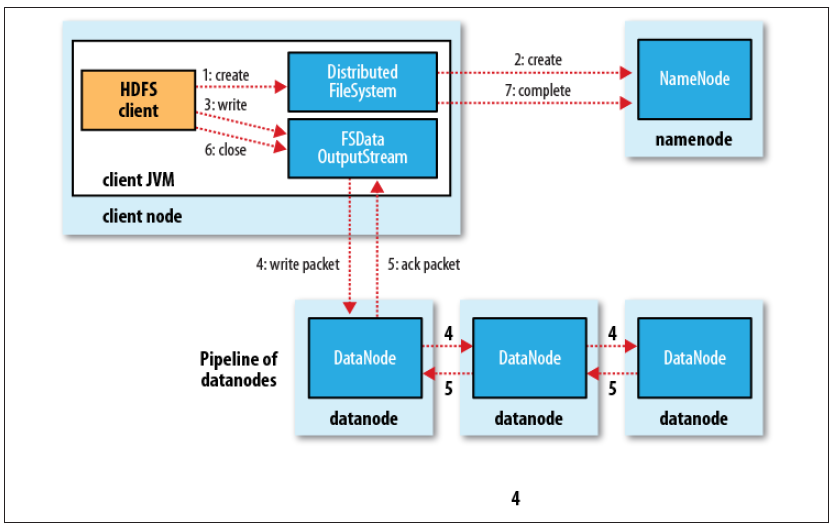
\includegraphics[width=\textwidth]{write.png}
\caption{\it Ghi dữ liệu trên HDFS \cite{write}}
\end{figure}
\end{itemize}

\subsubsection{Tổng quan về MapReduce}
Nhờ HDFS, ta đã có thể lưu trữ được lượng rất lớn dữ liệu với độ tin cậy cao. Tuy nhiên, vấn đề đặt ra là ta sẽ phải làm gì với những dữ liệu đấy? Xử lý nó ra sao? Làm thế nào để xử lý chúng được nhanh chóng? - Đó là lý do mà MapReduce được tạo ra.

Được bắt nguồn từ bài báo nổi tiếng của Google \cite{mapreduce_google}, nó là mô hình tính toán song song phân tán rất mạnh mẽ của Hadoop. MapReduce được coi là trái tim của Hadoop, dù mô hình tuy đơn giản, bao gồm hai hàm chính là map và reduce. 

Để hiểu MapReduce hoạt động như thế nào, ta bắt đầu với ví dụ sau: \\
Dữ liệu được lấy từ Trung tâm dữ liệu thời tiết của Mỹ (National Climatic Data Center). Được lưu trữ dưới dạng từng dòng văn bản ASCII, mỗi dòng một bản ghi, dưới dạng các file zip. Giả sử bắt đầu từ 1901 đến 2001. Dữ liệu được lưu trữ trên HDFS

\begin{figure} [H]
\centering
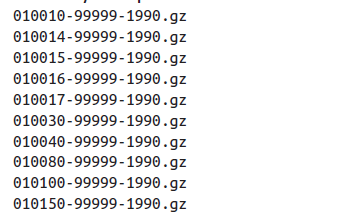
\includegraphics[width=7cm]{data.png}
\caption{\it Dữ liệu của năm 1990 được lưu trữ thành các file gzip}
\end{figure}

\begin{figure}[H]
\centering
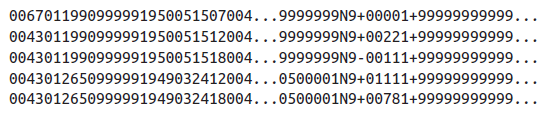
\includegraphics[width=11cm]{lines.png}
\caption{\it Ví dụ về một vài dòng dữ liệu}
\end{figure}

MapReduce bắt đầu khi Hadoop lựa chọn các datanode nơi các block của dữ liệu được lưu trữ.  Input Reader được chạy trên node đó, thực hiện search toàn bộ các file trong thư mục cần tính toán, đọc dữ liệu, trả về dưới dạng <key, value> (Ở đây key là số thứ tự dòng, value là mỗi dòng). Do dữ liệu được lưu ngay tại datanode nên việc đọc dữ liệu sẽ giống như đọc trên đĩa thông thường. 

\begin{figure}[H]
\centering
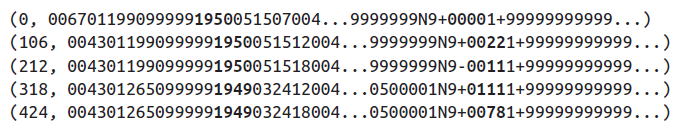
\includegraphics[width=14cm]{input_reader.png}
\caption{\it Dữ liệu sau khi qua Input Reader}
\end{figure}

Tiếp theo, hàm map được chạy nhiều lần trên datanode đó. Mỗi hàm map được thực hiện ứng với dữ liệu đầu vào là <key, value> của Input Reader, thực hiện phân tích, tách lấy <key, value> mới và trả về (Ở đây key là số năm, value là nhiệt độ), được sắp xếp theo key và lưu trữ các giá trị này trên ổ cứng.

\begin{figure}[H]
\centering
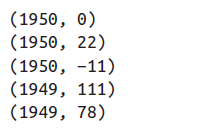
\includegraphics[width=4cm]{map.png}
\caption{\it Dữ liệu sau khi qua hàm map}
\end{figure}

Dữ liệu trên nhiều datanode sẽ được gửi qua mạng, tập hợp lại ở một vài node. Nhờ hàm shuffle, dữ liệu được ghép lại và sắp xếp một lần nữa:

\begin{figure}[H]
\centering
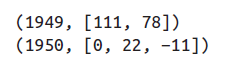
\includegraphics[width=5cm]{shuffle.png}
\caption{\it Dữ liệu sau khi qua hàm shuffle}
\end{figure}

Cuối cùng trên các node đấy sẽ gọi hàm reduce, nhận giá trị là key và một danh sách các giá trị đã ghép, thực thi và trả về <key, value> mong muốn (Ở đây hàm reduce sẽ tìm giá trị lớn nhất của nhiệt độ). Dữ liệu được lưu trữ trở lại HDFS dưới dạng một file kết quả.

\begin{figure}[H]
\centering
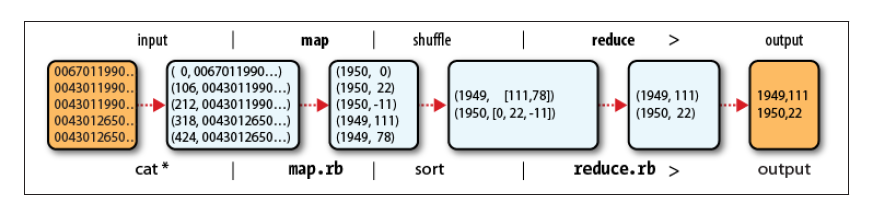
\includegraphics[width=\textwidth]{data_flow.png}
\caption{\it Dữ liệu qua các hàm MapReduce}
\end{figure}

\begin{figure}[H]
\centering
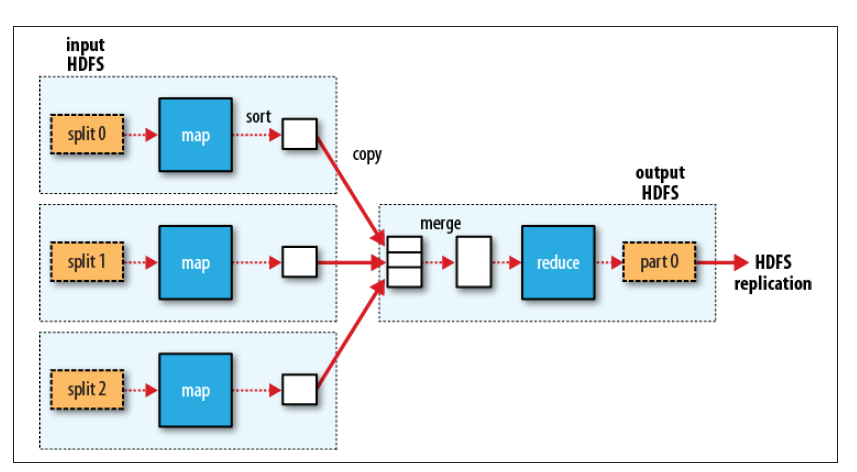
\includegraphics[width=\textwidth]{single_reduce.png}
\caption{\it Data flow với trường hợp một hàm reduce}
\end{figure}

\begin{figure}[H]
\centering
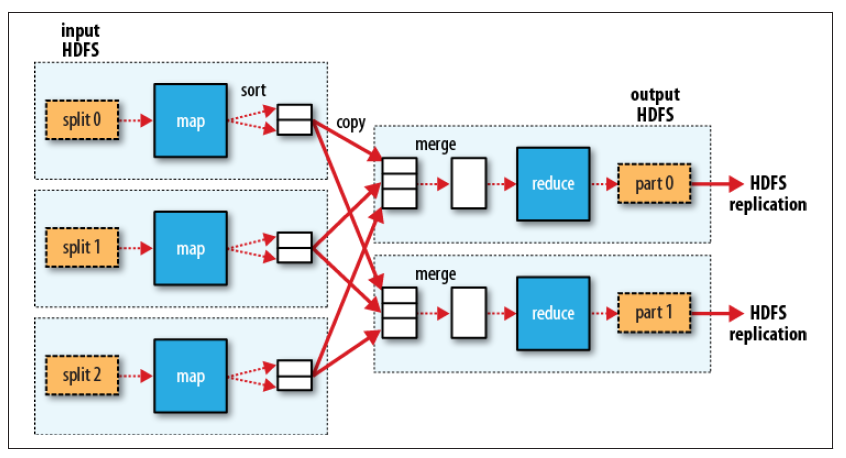
\includegraphics[width=\textwidth]{multi_reduce.png}
\caption{\it Data flow với trường hợp nhiều hàm reduce}
\end{figure}

Những ưu điểm của MapReduce so với các phương pháp tính toán thông thường:
\begin{itemize}
\item[+] Tính mở rộng
\item[+] Lời giải chi phí thấp
\item[+] Tính mềm dẻo
\item[+] Tốc độ cao nhờ tính toán song song

Được sử dụng rộng rãi trong nhiều ứng dụng, bao gồm việc tìm kiếm, sắp xếp, tính toán phân tán, học máy, … Tại google, nó được sử dụng cho việc sinh ra toàn bộ Google index của World Wide Web, phục vụ cho công cụ Search Engine mạnh mẽ của mình.
\end{itemize}

\chapter*{Cơ hội, thách thức và chỉ trích}
\addcontentsline{toc}{chapter}{Cơ hội, thách thức và chỉ trích}
\section*{Cơ hội}
\begin{itemize}
\item
Tiếp cận và nghiên cứu về dữ liệu lớn sẽ giúp cho chúng ta có thêm phương án giải quyết, xử lý và đối phó với những thách thức đối sản xuất số liệu thống kê chính thức trong hiện tại và tương lai. Những nghiên cứu thực nghiệm cần phải được tiến hành để khám phá những ứng dụng tiềm năng của dữ liệu lớn trong số liệu thống kê
chính thức, và nghiên cứu thực nghiệm đó phải là một phần trong quy trình sản xuất
số liệu thống kê.
\item
Nghiên cứu về dữ liệu lớn cần phải có cơ sở hạ tầng công nghệ thông tin hiện đại,
đáp ứng các yêu cầu xử lý khối lượng lớn dữ liệu và nhanh, đồng thời có thể tập hợp
dữ liệu từ nhiều nguồn khác nhau. Thực hiện được điều này chúng ta có được đội ngũ
nguồn nhân lực về quản lý và khai thác Big data vững vàng về chuyên môn và được
trải qua kinh nghiệm thực tế.
\item
Tiếp cận và nghiên cứu về dữ liệu lớn sẽ giúp chúng ta có được những văn bản
pháp lý bổ sung có thể giúp cho cơ quan thống kê chính thức có điều kiện để thực
hiện được khai thác dữ liệu thông qua hồ sơ hành chính, ngoài ra dữ liệu cũng được
bảo đảm và giữ bí mật nhờ những văn bản pháp lý bổ sung này.
\item
Sử dụng dữ liệu lớn đem lại niềm tin của cộng đồng với thống kê chính thức do
quá trình trình sản xuất số liệu thống kê chính thức với dữ liệu lớn hoàn toàn không có
sự tác động chủ ý của con người.
\end{itemize}

\section*{Thách thức, chỉ trích}
\begin{itemize}
\item \textbf{Khai thác và sử dụng}: Nhân viên khai thác chưa đủ mạnh dẫn đến việc giảm hiệu quả về giá trị của Big Data
so với ban đầu, dẫn đến lãng phí tài nguyên. Thực tế khi các công ty đã đầu tư hàng tỉ
USD vào Big Data và lấy được thông tin về nhiều thứ nhưng chỉ có ít hơn 40\% nhân
viên thật sự có thể hiểu và tận dụng các thông tin này. Nhiều đơn vị, tổ chức không đo
lường được vấn đề sẽ phát sinh trong quá trình triển khai thực hiện, dự toán kinh phí
chưa chính xác, do vậy dự án không thực hiện được.

\item \textbf{Quản lý}: Do luật pháp quy định sử dụng và khai thác ở mỗi quốc gia là khác nhau nên cách
quản lý là cũng khác nhau .Khoa học dữ liệu lớn đang phát triển mạnh trong những tổ
chức tư nhân, trong khi đó bộ phận này chưa được liên kết với những tổ chức của
chính phủ một cách chặt chẽ dẫn đến việc quản lý vẫn còn nhiều vướng mắc..

\item \textbf{Quyền riêng tư}: Người ta lo lắng về vấn đề quyền riêng tư của người dùng. Việc thu thập Big Data có
thể sẽ đi kèm thông tin có khả năng định dạng người dùng mà không được sự đồng ý
của họ, và điều đó vi phạm luật ở một số quốc gia. Nhiều chuyên gia từ nhiều lĩnh vực
khác nhau hiện đang thúc đẩy việc bảo vệ quyền riêng tư khi sử dụng Big Data.

\item \textbf{Phạm vi dữ liệu}: Để ý rằng nguồn dữ liệu từ big data là vô hạn. Tuy nhiên big data chỉ giúp miêu tả thế
giới trong quá khứ, hoặc tốt lắm là hiện tại. Việc sử dụng Big Data để nói về tương lai thì
cần phải kết hợp thêm với các phương pháp mô hình, mô phỏng hay nghiên cứu về sự
chuyển động của thế giới thì mới đưa ra dự đoán chính xác được.
\end{itemize}


\chapter*{Kết luận và hướng phát triển}
\addcontentsline{toc}{chapter}{Kết luận và hướng phát triển}

\begin{itemize}
\large
\it
\item[-] Kết luận về ưu nhược điểm: Đã làm hoặc chưa làm được gì.
\item[-] Hướng phát triển cho đề tài, cho sản phẩm và khả năng ứng dụng.
\end{itemize}

Đề tài đã đề cập tới khái niệm Big Data, đưa ra nhiều ví dụ để giải thích được mức độ quan trọng của Ưu điểm: Ứng dụng Bigdata trong cuộc sống. Đồng thời đã cũng đã chạm được vào cơ chế xử lý dữ liệu lớn để khai thác hiệu quả nguồn dữ liệu. Phân tích những vấn đề bất cập, liên quan đến đạo đức khoa học trong ứng dụng Big Data. 

Nhược điểm: Do phạm vi nội dung báo cáo có giới hạn, cùng với mong muốn hướng tới những đối tượng không chuyên, nên chưa đào sâu vào định lượng tính toán liên quan đến công nghệ xử lý dữ liệu lớn, mà chỉ đề cập tương đối định tính về vấn đề này.

Hướng phát triển cho đề tài: 

Ý tưởng: “Bàn làm việc mẫu mực!” \\
Ý tưởng này là thiết kế một bộ bàn ghế làm việc, trong đó chiếc ghế được gắn cảm biến có thể cảm nhận được tư thế ngồi của chủ nhân nó trong quá trình làm việc, chiếc ghế sẽ được kết nối mạng với máy tính hoặc smartphone của chủ sử dụng. Đồng thời cũng được kết nối mạng tới một máy chủ mạng được tích hợp dữ liệu lớn đã thu thập về mối quan hệ giữa tư thế ngồi và tình trạng sức khỏe của người sử dụng. Như vậy, khi làm việc, chủ nhân của chiếc ghế sẽ được đánh giá sơ bộ về cân nặng, chiều cao, rồi sau một thời gian làm việc, nếu người sử dụng có những tư thế thể hiện sự mệt mỏi, máy tính có thể hiện lên một dòng chữ nhẹ nhàng lướt qua, nhắc nhở chủ nhân nó hãy tỉnh táo lại hoặc “hãy nghỉ ngơi một chút, bạn đã ngồi làm việc quá lâu!”. Quan trọng hơn, khi tư thế ngồi của người sử dụng có thể ảnh hưởng tới cột sống, máy tính hay smartphone có thể nhắc nhở người sử dụng của nó nên điều chỉnh tư thế nếu không sẽ ảnh hưởng xấu tới sức khỏe. Chiếc bàn, dĩ nhiên được gắn cảm biến hồng ngoại, xác định được độ tỉnh táo của người sử dụng thông qua phân tích độ mở to của đôi mắt, phân tích độ sáng của không gian xung quanh để điều chỉnh độ sáng màn hình máy tính và đèn làm việc cho phù hợp. Và đồng thời xác định khoảng cách giữa mắt người và bàn làm việc để đảm bảo đôi mắt của người sử dụng được khỏe mạnh.

\begin{thebibliography}{30}
\bibitem{definition}
\textit{Big Data là gì và người ta khai thác, ứng dụng nó vào cuộc sống như thế nào?}, 2016. \\
\url{https://www.linkedin.com/pulse/big-data-l%C3%A0-g%C3%AC-v%C3%A0-ng%C6%B0%E1%BB%9Di-ta-khai-th%C3%A1c-%E1%BB%A9ng-d%E1%BB%A5ng-n%C3%B3-v%C3%A0o-cu%E1%BB%99c-nguyen}

\bibitem{top500}
\textit{The Supercomputer Landscape Today}, 2013. \\
\url{http://wiki.expertiza.ncsu.edu/index.php/CSC/ECE_506_Spring_2013/1b_dj}

\bibitem{hadoop}
\textit{Apache Hadoop}. \\
\url{https://en.wikipedia.org/wiki/Apache_Hadoop}

\bibitem{read}
Tom White (2015), \textit{Hadoop: The Definitive Guide}, 4th Edition, O'Reilly Media, page 69.

\bibitem{write}
Tom White (2015), \textit{Hadoop: The Definitive Guide}, 4th Edition, O'Reilly Media, page 72.

\bibitem{mapreduce_google} 
Jeffrey Dean and Sanjay Ghemawat, 2004, \textbf{\it MapReduce: Simplified Data Processing on Large Clusters}, Google, Inc. \\
\url{https://static.googleusercontent.com/media/research.google.com/vi//archive/mapreduce-osdi04.pdf}

\end{thebibliography}

\end{document}
